\providecommand{\atd}{..}
\documentclass[../ATD.tex]{subfiles}

\begin{document}
    \chapter{Installation setup}\label{ch:installation-setup}
    \section{References}\label{sec:references}
    The installation setup has been done by following the two documents provided by the developers of the system:
    \begin{itemize}
        \item SoftwareToInstall
        \item ITD1
    \end{itemize}
    Both the documents can be found on github, in the folder \href{https://github.com/gianfi12/AbboAccordiBonetti/tree/master/DeliveryFolder}{\emph{DeliveryFolder}}.

    \section{Installation choice}\label{sec:installation-choice}
    The following software has been used:
    \begin{itemize}
        \item \textbf{Glassfish5}: Glassfish has been used in its 5.0 version instead of the 4.0 (required in the ITD) because of an error that did not allowed to run the server (on iOS).
        The developer group ensured us that this choice was fine, since their team worked with that version too.
        Moreover, using Linux on another machine and Glassfish4, we could not deploy the web server(tried to deploy on console and on glassfish GUI, same error):

        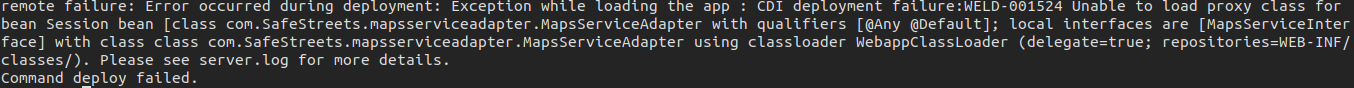
\includegraphics[scale = 0.35]{assets/deployError.png}

        \item \textbf{IntelliJ}: we used mainly IntelliJ to run the application, but some tests have been done even with AndroidStudio, to actually prove that
        IDE is not the problem.
    \end{itemize}
    \newpage
    \section{Installation issues}\label{sec:installation-issues}
    \subsection{iOS issues}\label{subsec:ios-issues}
    On our Apple machine,
    during the server deploy process, an issue that did not allow the application to communicate with the server came up.
    We have been able to solve it by communicating with the developers.
    The problem that we found was that the SafeStreetsSOAP and SafeStreetsWebServer were assigned to an unrecognized link, different from the once that were expected by the client.
    The expected links were \textit{\${com.sun.aas.instanceRootURI}/applications/SafeStreetsSOAP/} and \textit{\${com.sun.aas.instanceRootURI}/applications/SafeStreetsWebServer/},
    while we found \textit{\${com.sun.aas.instanceRootURI}/applications/SafeStreetsSOAP534859734543/} and \newline\textit{\${com.sun.aas.instanceRootURI}/applications/SafeStreetsWebServer54378953479583/}.
    \newline To solve the problem, we needed to go in the glassfish5/glassfish/domains/domain1/config folder and modify the domain.xml file by removing the unexpected characters wherever they show up and
    redeploy everything.

    \subsection{Linux issues}\label{subsec:linux-issues}
    On our Ubuntu machine,
    during the import of the file database.sql file, these issues came up:

    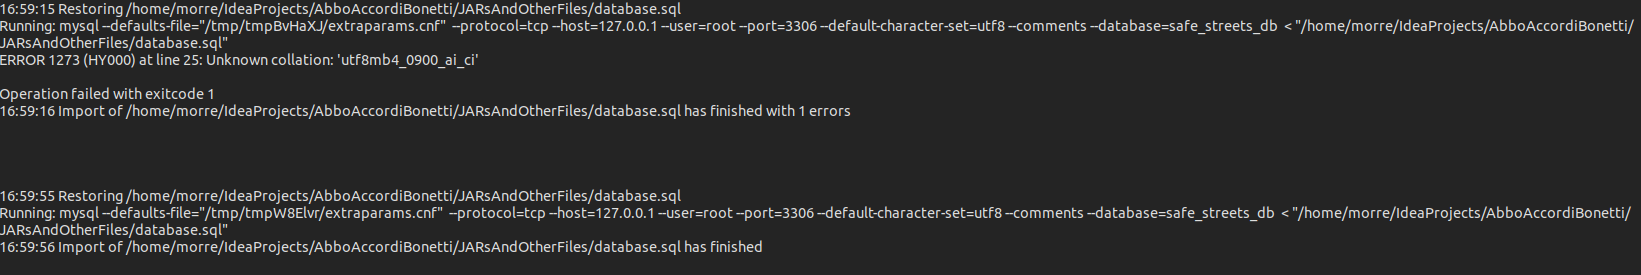
\includegraphics[scale = 0.3]{assets/errorDb.png}
    the error is: Unknown collation: 'utf8mb4\_0900\_ai\_ci' ,
    so we opened that sql file and changed all the occurrences of utf8mb4\_0900\_ai\_ci with utf8mb4\_general\_ci. \newline
    \\
    The only issue encountered during the deployment of the server is specified above (section 2.2), and was solved by using Glassfish5.


\end{document}